\section{Ground Based versus Space Based Telescopes} % (fold)
\label{sec:ground_based_versus_space_based_telescopes}
	Ground based telescopes are seeing limited which is a resolving limitation due to distortion caused by the atmosphere. Light is scattered by the atmosphere and so detecting a source by these telescopes can be difficult. There is also the limitation of considerably more background light, compared to what is measured by space telescopes. To minimise these limitations, ground based telescopes are usually located at high altitude at locations such as Mauna Kea, Hawaii. The main advantage of ground based telescopes is that they can be built to very large sizes with telescopes with a primary diameter of around 30\,metres on the periphery. This cannot be achieved by space telescopes as the cost of transport to space would be very large and the telescope may well be damaged during this transportation.

	Space based telescopes are diffraction limited, i.e.\ the only limitation is whether they can resolve the object being observed. Taking the source as a point spread function, the light from the source will spread out and so the telescope must determine the source. This is important as light from other sources in the sky may almost overlap and so the diffraction gives the angle in the sky which can be resolved. Thus if the diffraction angle, the smallest angle between two objects can be resolved, is small, the better the telescope. Should two sources fall within this diffraction angle when looking into the sky, the telescope will not be able to resolve the two objects and so one cannot be distinguished from another. The diffraction angle can be calculated using the formula below:
	\begin{align}
		\Delta\theta= \frac{(1.22 \lambda)}D
	\end{align}

	This also shows that the larger the diameter, the smaller the diffraction angle will be and so the better the telescope will be at resolving sources.

	The main disadvantage of space based telescope is that they must be transported into space. This is usually done with the aid of a rocket and so the cost of achieving this can be considerable. The telescope may also be damaged during this transportation and so this limits the size of the telescope as a smaller size will mean a smaller chance of being damaged. The James Webb Space Telescope scheduled for launch in 2018 consists of a 6.5 metre primary mirror made up of multiple mirrors that will unfold once it is in space. Despite this folding up of the telescope, the primary mirror size is still small relative to some ground based ones currently in use such as the VLT (primary mirror of 8.2\,metres) and is considerably smaller than some proposed for the future such as the EELT (primary mirror 39.3\,metres).


	\subsection{Astronomical Seeing} % (fold)
	\label{sub:astronomical_seeing}
		Plane waves from a source being observed are distorted by the Earth’s atmosphere and so upon reaching a telescope within the atmosphere are slightly perturbed and so the image formed is blurred. This effect is contributed to by numerous layers where different temperatures or the interaction of different wind speed causes this effect with ‘Seeing’ the term used to describe the total distortion of the wavefront\cite[page~188]{Diffraction_Limited_Imaging_Saha}. This effect is shown below in figure~\ref{fig:Seeing} where a turbulent layer of the atmosphere causes a change in the shape of the wavefront.
		\begin{figure}[ht]
			\centering
			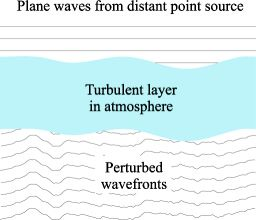
\includegraphics[width=0.4\textwidth]{../Images/Seeing.png}
			\caption{Figure 1}\label{fig:Seeing}
		\end{figure}

		Whilst the resolving power of a telescope is generally largely dependent on its diameter, this seeing limitation becomes the major source of error when resolving a point source from within the Earth’s atmosphere. This is consequently the main limitation for ground based telescopes which are therefore known as being seeing limited. A point spread function (PSF) imaged in these circumstances produces what is known as a seeing disc due to the atmospheric turbulence and the most common measurement used to describe this effect is the full width at half maximum, hereafter the FWHM, shown below in figure~\ref{fig:FWHM} where a peak shape is produced by this overall blurring of the source. When measuring the flux arriving at the CCD from a particular source, an area of radius four times the FWHM is recorded over and so a larger value of FWHM also increases the integration time required to observe the source.
		\begin{figure}[ht]
			\centering
			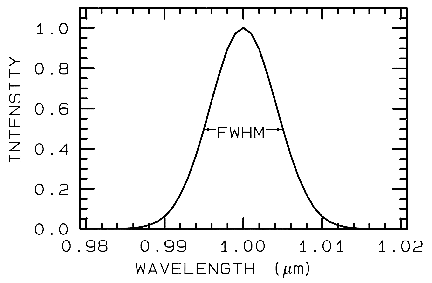
\includegraphics[width=0.5\textwidth]{../Images/FWHM.png}
			\caption{Figure 1}\label{fig:FWHM}
		\end{figure}
	% subsection astronomical_seeing (end)

	\subsection{The Future of Ground Based Telescopes} % (fold)
	\label{sub:the_future_of_ground_based_telescopes}
		The main disadvantage of ground based telescopes compared to space based telescopes is the poorer resolution due to the distortion caused by the atmosphere or astronomical seeing. The introduction of adaptive optics however, should help resolve this issue and allow ground based telescopes to be only diffraction limited similar to space based ones. This, combined with the large diameter mirrors currently in the pipeline such as for the European Extremely Large Telescope (E-ELT), a primary mirror of 39.3 metres, and the Giant Magellan Telescope (GMT), a primary mirror of 25\,metres, ensure ground based telescopes hold a place in the future of space observation, even if just to compliment space based ones. The larger mirrors ensure a greater light collecting power, receiving more photons for the source being observed and so significantly reducing the observing time required. These large diameter mirrors are currently only possible for ground based telescopes and so provide them with a distinct advantage over space based ones.

		\subsubsection{Adaptive Optics} % (fold)
		\label{ssub:adaptive_optics}
			As described earlier in astronomical seeing, light passing through the atmosphere from a source, such as a distant galaxy, is perturbed due to atmospheric turbulence and so the images produced by ground based telescopes are blurred. Adaptive optics works by first sensing the wavefront perturbations and then counteracting this blurring in real time thus enabling the telescopes to hold a much larger resolving power. This system will be used on future ground based telescopes ensuring they are no longer limited by the ability to resolve a source. An example of how this is set up, as on the Subaru Telescope, is shown below in figure~\ref{fig:AdaptiveOptics}.
			\begin{figure}[ht]
				\centering
				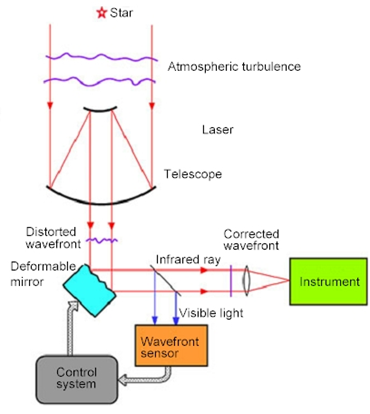
\includegraphics[width=0.6\textwidth]{../Images/AdaptiveOptics.png}
				\caption{Figure 1}\label{fig:AdaptiveOptics}
			\end{figure}

			The wavefront sensor (WFS) measures the distortions in the incoming wavefront of light. This then provides the measured information to an actuator control computer identified in figure~\ref{fig:AdaptiveOptics} as the control system. This then adjusts the shape of the adjustable mirror to effectively correct the wavefront reaching the telescope\cite{Diffraction_Limited_Imaging_Saha}.  The wavefront sensor can measure the distortions introduced into the wavefront on the timescale of a few milliseconds with the information then computed and the shape of the mirror adjusted accordingly. The correction process should therefore be completed in a time similar to the time between the changes of the wavefront thus ensuring the distortion is compensated for.
		% subsubsection adaptive_optics (end)
	% subsection the_future_of_ground_based_telescopes (end)
% section ground_based_versus_space_based_telescopes (end)


\section{Observation Times} % (fold)
\label{sec:observation_times}
	The main aim of this project is to produce an observing strategy to view some of the earliest galaxies in the universe. An important aspect of this is therefore the viewing of the galaxies themselves and the time it will take to do so. The time required to view these galaxies depends not only on the telescope being used, but also the devices used. A charged coupled device (CCD) will be used to measure the light from these sources and so to calculate the times required to view these galaxies, these must be understood in more detail. The telescope or telescopes used during the observation of these galaxies will have different properties which will affect the time required to view the source. Some of these are mentioned below.

	\subsection{Telescope Properties} % (fold)
	\label{sub:telescope_properties}

		\subsubsection{Mirror Reflectivity} % (fold)
		\label{ssub:mirror_reflectivity}
			One such factor that will increase the time required to view a source is the reflectivity of the mirrors used on the telescope. The mirror reflectivity, given as a percentage, is the amount of light reflected by the mirror. Some of the light is absorbed as the mirror is not one hundred per cent efficient meaning not all photons striking the mirror reach the CCD. The reflectivity differs depending on the material used on the surface of the mirrors. Various optical coatings are produced and used depending on the wavelengths being observed, for example, the James Webb Space Telescope uses a gold coating which is particularly useful in the infrared region and also very durable due to the inert nature of Gold. The reflectivity of this gold coated mirror is in the region of 98--99\%\cite{Quantum_Coatings_Incorporated}. Other coatings regularly used include aluminium, which has a reflectivity in the region of 80--90\% and is utilised in the UV and IR range, as well as silver, which has a reflectivity in the range of 95--99\% and is utilised in the visible and IR range.
		% subsubsection mirror_reflectivity (end)

		\subsubsection{Telescope Throughput} % (fold)
		\label{ssub:telescope_throughput}
			The definition of throughput is the ratio of the flux detected by a particular instrument in a given filter and the incoming flux measured over an area equal to the area of the telescope primary mirror\cite{WIRCam_Throughput}. The throughput is therefore the percentage of photons striking the primary mirror that reach the CCD and are recorded. This contributes to the time required to observe a source as not all the photons striking the primary mirror, originated from the source, will reach the CCD. As the number of photons reaching the CCD is fewer, a larger portion of time is required to obtain the sought after signal-to-noise ratio and so the overall observation lasts a longer period of time.
		% subsubsection telescope_throughput (end)

		\subsubsection{Filters}

		\subsubsection{Field of View}
	% subsection telescope_properties (end)

	\subsection{Charged Coupled Devices} % (fold)
	\label{sub:charged_coupled_devices}
		Describe CCD and how it works here.

		The CCD does however have numerous errors known as noise, which contribute to the integration time required to view these early galaxies and so must be taken into account. The conversion of light to pixel values in a CCD leads to an inevitable noise being introduced into the image. This noise is the unwanted variations in pixel values and causes the image produced to differ from the one being observed. The noise incurred will make it more difficult to distinguish the source being observed hence increasing the integration time. For an electrical measuring system such as a CCD, a signal to noise ratio characterises the quality of the measurement taken where the signal to noise ratio (SNR) is the ratio of signal from the source being observed and signal produced by background radiation and other sources of noise. This is generally used to quantify the quality of a CCD measurement. The main sources of noise for a CCD are the dark current, sky background and read noise, which are all described below.
	% subsection charged_coupled_devices (end)

	\subsubsection{Dark Current} % (fold)
	\label{ssub:dark_current}
		Atoms in the silicon substrate of the CCD used are thermally excited and thus electrons are freed. This occurs even when the CCD is not exposed to light, hence there is a steady creation of electrons, and this is called the dark or thermal current. As this is caused by thermal excitation, it strongly depends on the temperature at which the device is operating. At any given temperature, the rate at which electrons are freed is constant, however for every rise in temperature of 6 degrees Celsius, the dark current produced approximately doubles\cite[pages~124--125]{Astronomical_Image_Processing}. This relationship is shown in figure~\ref{fig:dark_current} below\cite{Southern_Observatory_throughput}.
		\begin{figure}[ht]
			\centering
			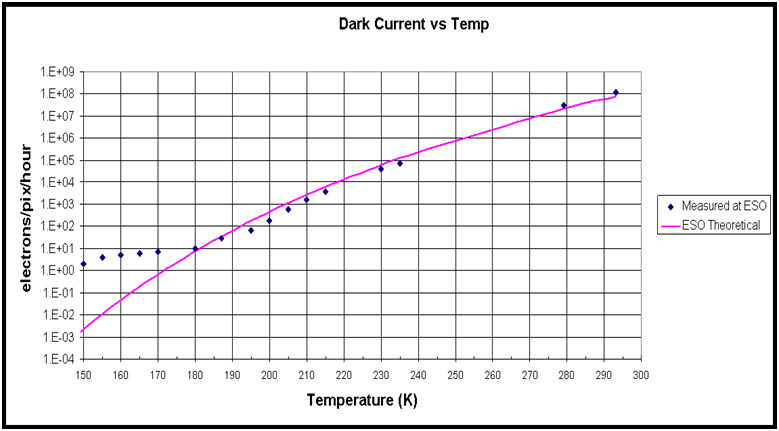
\includegraphics[width=0.7\textwidth]{../Images/Dark.png}
			\caption{Figure 1}\label{fig:dark_current}
		\end{figure}

		Figure 1 shows that relationship between temperature and dark current for a custom designed CCD provided to the European Southern Observatory and shows clearly the increase in dark current at higher temperatures. CCD’s are therefore cooled, often with the use of liquid nitrogen, to minimise this effect. The dark current itself is a relatively small electric current that flows through numerous photosensitive devices, and is one of the main sources of noise for a CCD.
	% subsubsection dark_current (end)

	\subsubsection{Sky Background} % (fold)
	\label{ssub:sky_background}
		The sky background is the incoming light from the sky measured on the telescope that is not from the source being observed. The amount of sky background can vary at different wavelengths and is mainly due to light diffusion by the atmosphere. There are numerous sources that contribute towards the sky background such as airglow and zodiacal light. Airglow is the atmospheric emission of photons at wavelengths from the near-UV to the near-IR range due to chemical reactions in the upper atmosphere\cite[page~9]{atmospheric_radiation_model}. These chemical reactions lead to light emission due to the decay of electrons from an excited state in one of the reaction products. One such example is the emission in the near infrared region by OH radicals created from a reaction between ozone and hydrogen in the upper atmosphere\cite{residual_OH_emission}. Other processes contributing to airglow are the recombination of ions originally ionised by the sun, and the luminescence of cosmic rays striking the upper atmosphere. Thermal radiation in the atmosphere by greenhouse gases also contributes to the sky background and is due to the absorption and emission of radiation from the Sun into the atmosphere in the mid-IR region. In this case, observations in the mid- and far-IR region must be carried out from outside the atmosphere\cite[pages~22--23]{Peter_Schneider_IR}. The sky background is therefore primarily an issue for ground based telescopes as they can incur a large background number of photons compared to the number of photons arriving from the source being observed. As space based telescopes are situated outside of the atmosphere, they avoid almost all of this background.
	% subsubsection sky_background (end)
% section observation_times (end)

